\section{Model for count data}



\begin{frame}[fragile]
  \frametitle{Motivations: oak powdery mildew pathobiome}

  \begin{block}{Metabarcoding data from [JFS16]}<1->
    \begin{itemize}
    \item $n = 116$ leaves, $p = 114$ species ($66$ bacteria, $47$ fungies + \textit{E. alphitoides})
\begin{knitrout}
\definecolor{shadecolor}{rgb}{0.969, 0.969, 0.969}\color{fgcolor}\begin{kframe}
\begin{alltt}
\hlstd{counts[}\hlnum{1}\hlopt{:}\hlnum{3}\hlstd{,} \hlkwd{c}\hlstd{(}\hlnum{1}\hlopt{:}\hlnum{4}\hlstd{,} \hlnum{48}\hlopt{:}\hlnum{51}\hlstd{)]}
\end{alltt}
\begin{verbatim}
##       f_1 f_2 f_3 f_4 E_alphitoides b_1045 b_109 b_1093
## A1.02  72   5 131   0             0      0     0      0
## A1.03 516  14 362   0             0      0     0      0
## A1.04 305  24 238   0             0      0     0      0
\end{verbatim}
\end{kframe}
\end{knitrout}
    \item $d = 8$ covariates (tree susceptibility, distance to trunk, orientation, \dots)
\begin{knitrout}
\definecolor{shadecolor}{rgb}{0.969, 0.969, 0.969}\color{fgcolor}\begin{kframe}
\begin{alltt}
\hlstd{covariates[}\hlnum{1}\hlopt{:}\hlnum{3}\hlstd{, ]}
\end{alltt}
\begin{verbatim}
##               tree distTOtrunk distTOground pmInfection orientation
## A1.02 intermediate         202        155.5           1          SW
## A1.03 intermediate         175        144.5           0          SW
## A1.04 intermediate         168        141.5           0          SW
\end{verbatim}
\end{kframe}
\end{knitrout}
    \item Sampling effort in each sample (bacteria $\neq$  fungi)
\begin{knitrout}
\definecolor{shadecolor}{rgb}{0.969, 0.969, 0.969}\color{fgcolor}\begin{kframe}
\begin{alltt}
\hlstd{offsets[}\hlnum{1}\hlopt{:}\hlnum{3}\hlstd{,} \hlkwd{c}\hlstd{(}\hlnum{1}\hlopt{:}\hlnum{4}\hlstd{,} \hlnum{48}\hlopt{:}\hlnum{51}\hlstd{)]}
\end{alltt}
\begin{verbatim}
##       f_1  f_2  f_3  f_4 E_alphitoides b_1045 b_109 b_1093
## [1,] 2488 2488 2488 2488          2488   8315  8315   8315
## [2,] 2054 2054 2054 2054          2054    662   662    662
## [3,] 2122 2122 2122 2122          2122    480   480    480
\end{verbatim}
\end{kframe}
\end{knitrout}
    \end{itemize}
  \end{block}

\end{frame}

\begin{frame}
  \frametitle{Problematic \& Basic formalism}
  
  \begin{block}{Data tables: $\bY = (Y_{ij}), n \times p$;  $\bX = (X_{ik}), n \times d$; $\bO = (O_{ij}), n \times p$ where}
    \vspace{-.25cm}
    \begin{itemize}
    \item $Y_{ij} = $ abundance (read counts) of species (genes) $j$ in sample $i$
    \item $X_{ik} = $ value of covariate $k$ in sample $i$
    \item $O_{ij} = $ offset (sampling effort) for species $j$ in sample $i$
    \end{itemize}
  \end{block}

  \vfill

  \begin{block}{Need for multivariate analysis to}
    \vspace{-.25cm}
    \begin{itemize}
    \item understand \emphase{between-species/genes interactions} \\
      \rsa 'network' inference (variable/covariance selection)
    \item correct for technical and \emphase{confounding effects} \\
      \rsa account for covariables and sampling effort
    \end{itemize}
  \end{block}

  \rsa need a generic framework to \alert{model dependences between count variables}

\end{frame}

%====================================================================

\begin{frame}{Models for multivariate count data}

  \begin{block}{If we were in a Gaussian world, the \alert{general linear model} would be appropriate}<1->
    For each sample $i = 1,\dots,n$, it explains 
    \begin{itemize}
    \item the abundances of the $p$ species ($\bY_i$) 
    \item by the values of the $d$ covariates $\bX_i$ and the $p$ offsets $\bO_i$
    \end{itemize}
    \begin{equation*}
      \bY_i = 
      \underbrace{\bX_i \mathbf{B}}_{\begin{tabular}{c} \text{account for} \\ \text{covariates}  \end{tabular}} 
      + \underbrace{\bO_i}_{\begin{tabular}{c} \text{account for} \\ \text{sampling effort}  \end{tabular}}
      \ + \bvarepsilon_i, 
      \ \bvarepsilon_i \sim \mathcal{N}(\bzr_p, \underbrace{\bSigma}_{\begin{tabular}{c} \text{\emphase{dependence}} \\ \text{\emphase{between species}}  \end{tabular}})
    \end{equation*}
    \begin{itemize}
      \item[\textcolor{mred}{+}] \only<1>{\emphase{null covariance $\Leftrightarrow$ independence \rsa uncorrelated species do not interact}}
      \only<2>{\sout{\emphase{null covariance $\Leftrightarrow$ independence \rsa uncorrelated species do not interact}}}
    \end{itemize}
  \end{block}

  \begin{block}{But we are not, and there is no generic model for multivariate counts}<2>
    \begin{itemize}
      \item Data transformation ($\log{}, \sqrt{} $) : quick and dirty \\
      \item Non-Gaussian multivariate distributions: do not scale to data dimension yet \\
      \item \emphase{Latent variable models}: interaction occur in a latent (unobserved) layer\\
    \end{itemize}
  \end{block}
    
\end{frame}

%====================================================================
\begin{frame}{{P}oisson-log normal (PLN) distribution}

  \begin{block}{A latent Gaussian model}<1>
  Originally proposed by Atchisson [AiH89]
  \[
    \bZ_i \sim \mathcal{N}(\bzr, \boldsymbol\Sigma)
  \]
  \[
    \bY_i \,|\, \bZ_i \sim \clP(\exp{\{\alert{\bO_i + \bX_i^\intercal \bB} + \bZ_i\}})
  \]
  \end{block}

  \vfill

  \begin{block}{Interpretation}
    \vspace{-.25cm}
  \begin{itemize}
   \item Dependency structure encoded in the latent space (i.e. in $\bSigma$)
   \item Additional effects are fixed
   \item Conditional Poisson distribution = noise model
  \end{itemize}
  \end{block}

  \begin{block}{Properties}
    \vspace{-.25cm}
      \begin{itemize}
        \item[\textcolor{green}{+}] over-dispersion
        \item[\textcolor{green}{+}] covariance with arbitrary signs
        \item[\textcolor{mred}{-}] maximum likelihood via EM algorithm is limited to a couple of variables
      \end{itemize}
  \end{block}

\end{frame}

%%%%%%%%%%%%%%%%%%%%%%%%%%%%%%%%%%%%%%%%%%%%%%%%%%%%%%%%%
\begin{frame}{Geometrical view}

\begin{knitrout}
\definecolor{shadecolor}{rgb}{0.969, 0.969, 0.969}\color{fgcolor}\begin{kframe}


{\ttfamily\noindent\bfseries\color{errorcolor}{\#\# Error in group\_by(observation, x, y): could not find function "{}group\_by"{}}}

{\ttfamily\noindent\bfseries\color{errorcolor}{\#\# Error in dplyr::summarize(obs, count = n()): object 'obs' not found}}

{\ttfamily\noindent\bfseries\color{errorcolor}{\#\# Error in ggplot(obs, aes(x, y)): object 'obs' not found}}

{\ttfamily\noindent\bfseries\color{errorcolor}{\#\# Error in eval(expr, envir, enclos): object 'p.observation.only' not found}}

{\ttfamily\noindent\bfseries\color{errorcolor}{\#\# Error in grid.arrange(p.latent + labs(x = "{}species 1"{}, y = "{}species 2"{}), : could not find function "{}grid.arrange"{}}}\end{kframe}
\end{knitrout}

\end{frame}

\begin{frame}
  \frametitle{Our contributions}

  \begin{block}{Algorithm/Numerical}
    A variational approach coupled with convex optimization techniques suited to higher dimensional data sets.
    
    \paragraph{{\tt PLNmodels} R/C++-package:}  \text{\url{https://github.com/jchiquet/PLNmodels}}
  \end{block}
  
  \vfill
  
  \begin{block}{Extensions for multivariate analysis}
     \paragraph{Idea:} put some additional constraint on the residual variance.
      \begin{itemize}
      \item \emphase{Network Inference} \\
        \rsa select direct interaction in $\bSigma^{-1}$ via sparsity constraints
        
      \item \textcolor{gray}{\it Principal component analysis}\\
        \textcolor{gray}{\it constraint the rank of $\bSigma$ (most important effect in the variance)}

    \end{itemize}

    \paragraph{Challenge:} a variant of the variational algorithm is required for each model
  \end{block}


\end{frame}

\begin{knitrout}
\definecolor{shadecolor}{rgb}{0.969, 0.969, 0.969}\color{fgcolor}\begin{kframe}


{\ttfamily\noindent\itshape\color{messagecolor}{\#\# \\\#\# Attaching package: 'igraph'}}

{\ttfamily\noindent\itshape\color{messagecolor}{\#\# The following objects are masked from 'package:stats':\\\#\# \\\#\#\ \ \ \  decompose, spectrum}}

{\ttfamily\noindent\itshape\color{messagecolor}{\#\# The following object is masked from 'package:base':\\\#\# \\\#\#\ \ \ \  union}}\end{kframe}
\end{knitrout}

\begin{frame}[fragile]
  \frametitle{PLN-network: unravel important interactions}

  \paragraph{Variable selection of direct effects.}
    \begin{align*}
      \bZ_i \text{ iid} & \sim \clN_p(\bzr_p, \bSigma), & \emphase{\|\bSigma^{-1}\|_1 \leq c} \\
      \bY_i \,|\, \bZ_i & \sim \clP(\exp\{\bO_i + \bX_i \bbeta + \bZ_i\})
      \end{align*}

  \paragraph{Interpretation: conditional independence structure.}
    \begin{equation*}
      (i,j)  \notin  \mathcal{E}  \Leftrightarrow  Z_i  \indep  Z_j  |
      Z_{\backslash \{i,j\}} \Leftrightarrow \bSigma_{ij}^{-1} = 0.
    \end{equation*}

    \begin{center}
      \begin{tabular}{c@{\hspace{2cm}}c}
        \begin{tabular}{c}
          \small $\mathcal{G}=(\mathcal{P},\mathcal{E})$ \\
          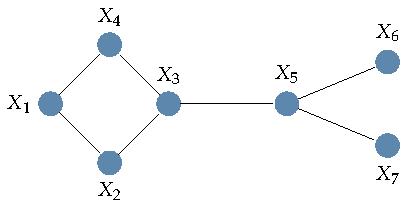
\includegraphics[width=.3\textwidth]{graph}
        \end{tabular}
     &
       \begin{tabular}{c}
         \small $\bSigma^{-1}$\\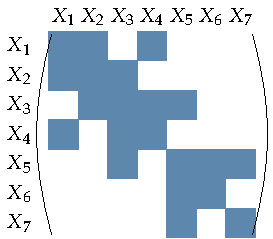
\includegraphics[width=.2\textwidth]{Markovadjacency}
       \end{tabular}
      \end{tabular}
    \end{center}

  \paragraph{PLN-network: find a sparse reconstruction of the latent inverse covariance}
  
    Iterate over variational estimator and Graphical-Lasso [BDE08,YL08,FHT07] in the latent layer

\end{frame}

\begin{frame}[fragile]
  \frametitle{Networks of partial correlations for oak mildew pathobiome}

\begin{knitrout}
\definecolor{shadecolor}{rgb}{0.969, 0.969, 0.969}\color{fgcolor}\begin{kframe}
\begin{alltt}
  \hlcom{# Models with offset and covariates (tree + orientation)}
  \hlstd{formula} \hlkwb{<-} \hlstd{counts} \hlopt{~} \hlnum{1} \hlopt{+} \hlstd{covariates}\hlopt{$}\hlstd{tree} \hlopt{+} \hlstd{covariates}\hlopt{$}\hlstd{orientation} \hlopt{+} \hlkwd{offset}\hlstd{(}\hlkwd{log}\hlstd{(offsets))}
  \hlstd{fits} \hlkwb{<-} \hlkwd{PLNnetwork}\hlstd{(formula,} \hlkwc{penalties} \hlstd{=} \hlnum{10}\hlopt{^}\hlkwd{seq}\hlstd{(}\hlkwd{log10}\hlstd{(}\hlnum{2}\hlstd{),} \hlkwd{log10}\hlstd{(}\hlnum{0.6}\hlstd{),} \hlkwc{len} \hlstd{=} \hlnum{30}\hlstd{))}
\end{alltt}
\end{kframe}
\end{knitrout}

\begin{knitrout}
\definecolor{shadecolor}{rgb}{0.969, 0.969, 0.969}\color{fgcolor}\begin{kframe}


{\ttfamily\noindent\bfseries\color{errorcolor}{\#\# Error in lapply(X = X, FUN = FUN, ...): object 'fits' not found}}

{\ttfamily\noindent\bfseries\color{errorcolor}{\#\# Error in eval(expr, envir, enclos): object 'fits' not found}}\end{kframe}
\end{knitrout}
\begin{overprint}
  \foreach\x in{1,...,15}{
    \includegraphics<\x>[trim={2.5cm 2.5cm 2.5cm 2.5cm},clip, width=\textwidth]{figures/plot-networks-\x}
  }
\end{overprint}

\end{frame}
